\section{Product \& Service Offering}
Our bottle has been engineered by students from UNIBO. The idea came after a cold meal at the university, and we started to think about how this issue can be solved without using those uncool food heaters that have to be plugged into the car plug.\\
The modern USB-C plug is what we were looking for: easy to use, widely spread and robust. Thanks to modern computers chargers it can also achieve a great amount of power (100W). The USB-C plug can also be used on the go with a power-bank.\\
This is already an interesting idea, but we made a step forward and decided to ride the wave of the reusable water bottles market, so we combined the attractive design of these ones, with our new product, keeping in mind the needs of our costumer.\\
The union between these two products is our BottAll, the all in one solution that takes over the original launch box and update it.\\
The product consists in three main pieces that can be screwed together, one over the other with a screw mechanism and a cap:
\begin{itemize}
\item \textbf{The water bottle}: just like other bottles on the market, It has a shielded metal surface that keeps the water fresh or cold for respectively 18 and 12 hours, and it can store up to 0.5l of liquid. In the bottom part we added a screw thread that let the costumer assemble it with the food box. 
\item \textbf{The food box}: this is a modern and attractive version of the classic plastic box: it is made by two metal layers to keep the inner temperature stable for approximately 3-4 hours. The capacity is 0.45l, it is suitable for approximately 100-120g of pasta. In the lower part there is an USB type-c which gives energy to the internal heater: according to the USB supply power, this will warm up the food and it can monitor the temperature via Bluetooth at the same time.
\item \textbf{Two cap}: are used in our product, one simple for the water, and one for the food box. The first one is a simple anti spill water cap, the second is designed by us to guarantee zero oil spill, and it has built in reusable cutlery locked by an hygienic cap. 
\end{itemize}
An important feature of the BottAll is the App which will be available in every app-store. With BottApp you can keep an eye on food temperature,
 and the internal power statistics. It can help to improve the health style of the costumer that can keep track of the food he eats and receive some healthy advices or recipes to bring with our product.
\subsection{Safety Requirements}
\begin{itemize}
\item The USB plug is rated IP67, so it can be easily washed with water and soap. 
\item Regulation (EC) No. 1935/2004 on materials and articles intended to come into contact with food and repealing Directives. %materials compliant with directives
\item Directive 2001/95/CE for general product security.
\end{itemize}

\subsection{Technology}
The technology behind the bottle and the food container is rather simple: all the parts are made by stainless steel, 100\% recyclable and infinitely reusable. Stainless steel is also durable and safe which makes it the best material for water transportation and storage. It is also widely used for city's water supply.\\
The heater on the bottom is an advanced and technological hardware: it features the latest USB-C connector and the Bluetooth connectivity, making it attractive and modern. Here we list the cutting-edge specs used: 
\begin{itemize}
\item Standard USB-C connector
\item Bluetooth low energy
\item 25W heater
\end{itemize}

\fullboxbegin
\begin{center}
HOW MUCH is 25W for heating my food??
\end{center}
$$Q=m\cdot c\cdot ∆t=0.2\si{\kilo\gram}\cdot 4180\cdot (50-25\si{\celsius})=20900\si{j}≈5.8 \si{Wh}$$
According to~\cite{sugo_e_pasta} the correct ratio of sauce to pasta is 3/2.
So, using 25W, it takes 14 minutes to heat up 80g of pasta and 120g of sauce from 25°C to 50°C.~\cite{energia_pasta}
\fullboxend
The BottAll bottle will connect with smartphone via BottApp. The operation diagram is shown right below:

\begin{figure}[H]
\centering
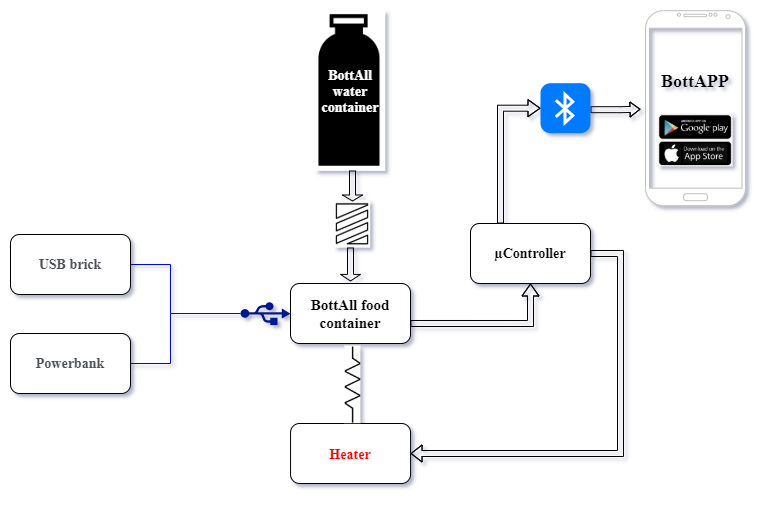
\includegraphics[width=0.7\textwidth]{images/bottigl1-block-diagram2.png}
\caption{BottAll Block Diagram}
\end{figure}

\subsection{How can i buy one}
During the first stage of the commercialization, our product will be available exclusively online thanks to the kick-starter campaign.\\
After first sales, it will be possible to buy it in our personal web store or in other physical shops in the Italian territory.\\
BottAll will be available in our online store with different options:
\begin{itemize}
\item Water plus food dispenser 
\item Only water 
\item Only food dispenser
\end{itemize}
\subsection{Protection}
Both the custom circuit and the BottApp will be design patented.
\subsection{Pricing Strategy}
Our goal is to sell the whole product, both water bottle and food container in the same package, but we will not neglect the possibility to buy them separately, both for replacement (to change colour/style) or by a standalone purchase. Just like other water bottles on the market, our aim is to build a stylish brand, so BottAll will be sold in standard colours, or more stylish pattern, subdividing market and prices. Prices will be better described in \cref{pricing}

\begin{table}[H]
\centering
\caption{Prices (euro)}
\begin{tabular}{cccc}
\toprule
& Only Water & Only Food & Both\\
\hline
Price & 25 & 40 & 55 \\
%Special Edition & 30 & 45 & 60 \\
\bottomrule
\end{tabular}
\end{table}

\subsection{What will it look like}
In \cref{fig:rendering}(a) you can have a look at the exploded view of the product, with an emphasis on the modularity.\\
In \cref{fig:rendering}(b) the collapsed view.
\begin{figure}[H]
    \centering
    \subfloat[\centering Exploded]{{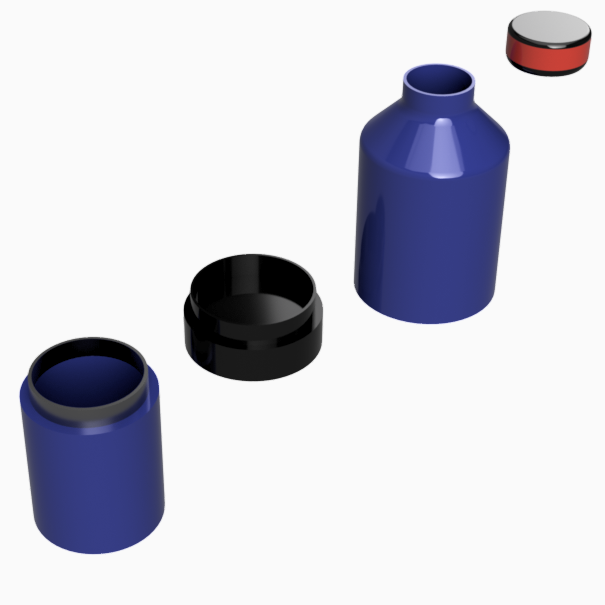
\includegraphics[width=0.45\textwidth]{images/esploso2.png} }}%
    \qquad
    \subfloat[\centering Collapsed]{{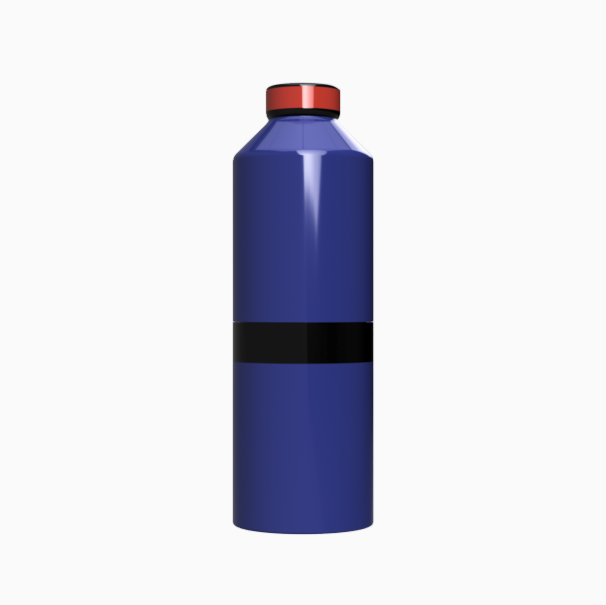
\includegraphics[width=0.45\textwidth]{images/intero2.png} }}%
    \caption{BottAll rendering}%
    \label{fig:rendering}
\end{figure}

At the bottom of the food container will be stored the circuit board provided with the cutting edge technologies we discussed before.
\begin{figure}[H]
\centering
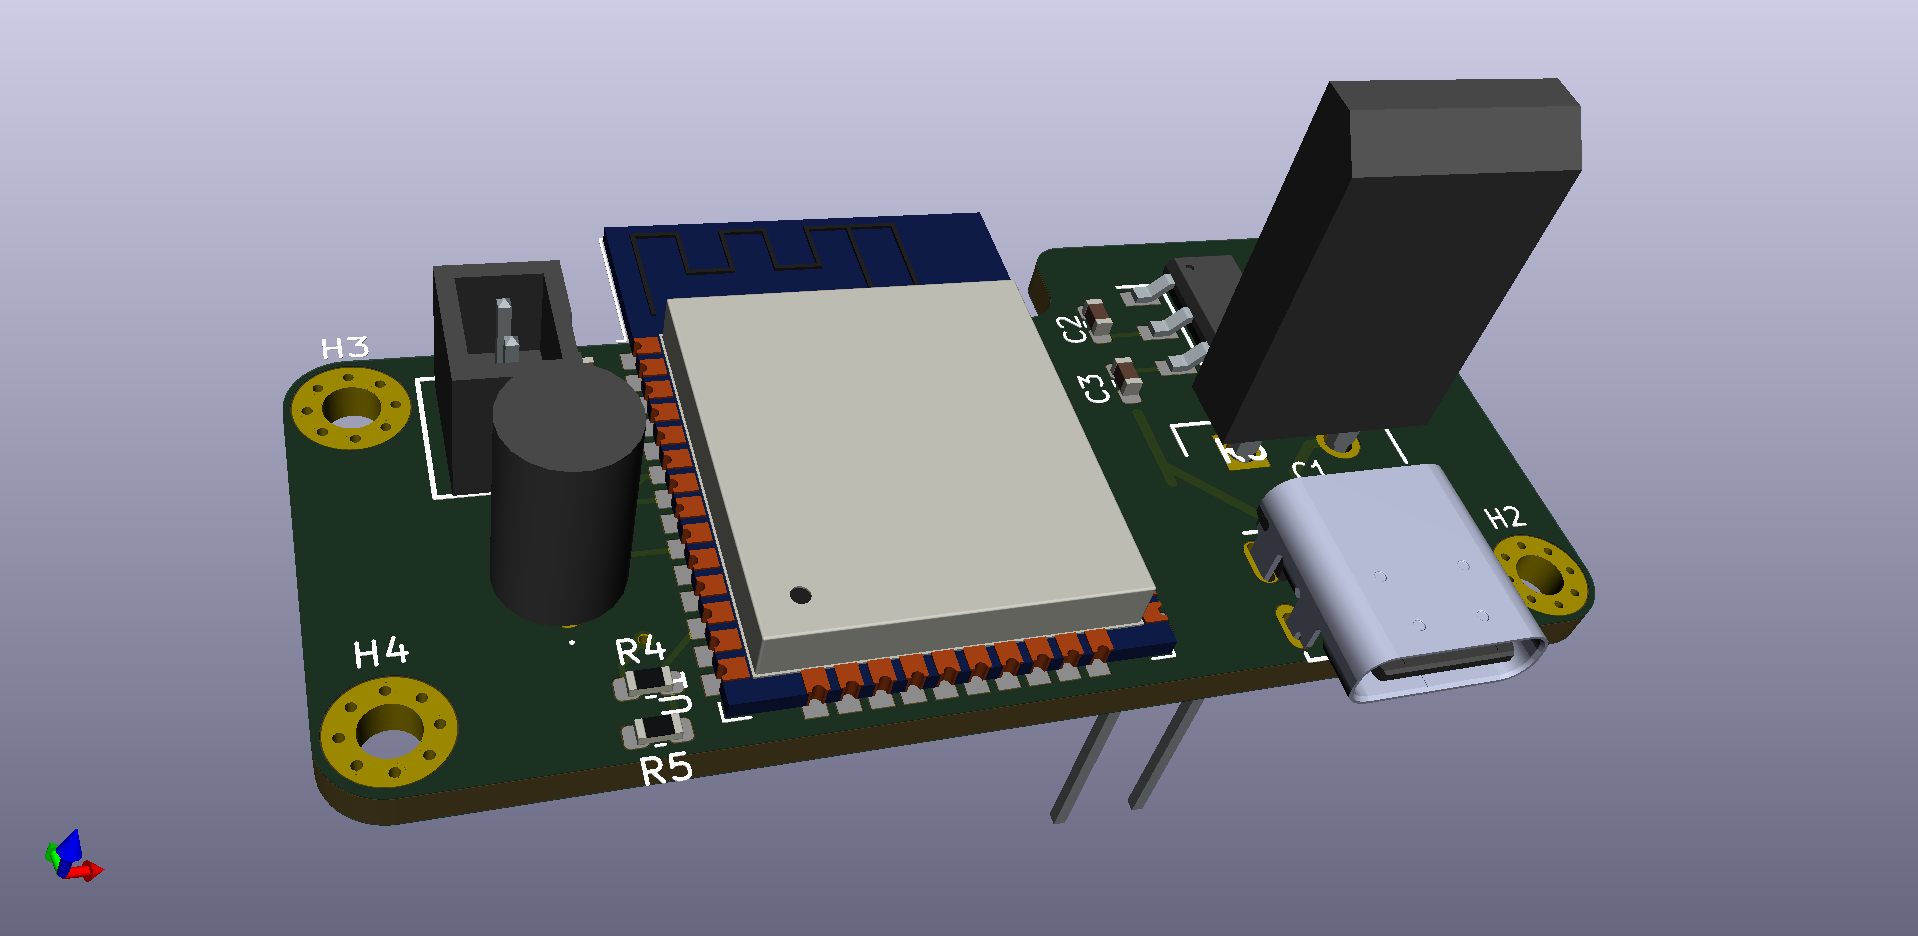
\includegraphics[width=0.5\textwidth]{images/circuito-scalda-vivande2.png}
\caption{BottAll Heater Board}
\end{figure}